% TODO: When to use bullets and when not?

\documentclass{article}

\usepackage{graphicx}
\usepackage{xcolor}

\definecolor{tempborder}{rgb}{1, 1, 1} % hide temp borders
%\definecolor{tempborder}{rgb}{0.9, 0, 0.9} % show temp borders

\definecolor{strongblue}{rgb}{0.2, 0.3, 0.7} % main theme color

\usepackage{hyperref}
\hypersetup{
    colorlinks=true,
    linkcolor=strongblue,
    filecolor=magenta,      
    urlcolor=strongblue,
}

\usepackage{pgfpages}
\usepackage{tikz}
\usetikzlibrary{calc}
\usetikzlibrary{matrix}
\usetikzlibrary{positioning}
\usepackage[active,tightpage]{preview}

\pgfdeclarelayer{background}
\pgfsetlayers{background,main}

\begin{document}
\begin{preview}

\def \mywebsite{https://mohnjahoney.github.io}



% Set independent lengths
\newcommand{\sidebarwidth}{6cm} % width of thin sidebar that runs down the side
\newcommand{\headerheight}{6cm} % height of header containing name and contact
\newcommand{\splitradius}{0.5cm} % split circle separates the four quadrants

\newcommand{\sectionpad}{0.3cm} % separation between section header and section and v.v.

\newcommand{\vennrad}{3cm}

% Compute dependent lengths
% TODO: need to include line widths?
% TODO: I think inner sep in the text blocks is messing with things.
\pgfmathsetlengthmacro\bodywidth{\pdfpagewidth - \sidebarwidth - 2*\splitradius}
\pgfmathsetlengthmacro\bodyheight{\pdfpageheight - \headerheight - 2*\splitradius}

%%% TIKZPICTURE
\begin{tikzpicture} [
mat/.style={draw=tempborder, rectangle, matrix of nodes, rounded corners, line width=0pt, inner sep=0pt, outer sep=0pt},
sec_title_mat/.style={mat, draw=none, fill=white},%, text width=, text depth=}, % use matrix for organizing each section
sec_body_mat/.style={mat, draw=none, fill=strongblue!10!white},%, text width=, text depth=}, % use matrix for organizing each section
sec_title/.style={font=\Large}, % section title
sec_title_circle/.style={draw=strongblue, circle, line width=2pt, minimum width=0.2cm, anchor=center}, % circles used to demarkate section titles
sec_bold/.style={font=\bfseries\normalsize, inner sep=3pt}, % bold "bullets" within each section
sec_text/.style={font=\normalsize, inner sep=3pt}, % main text in each section
sidebar_text/.style={font=\large, inner sep=3pt}, % main text in each section
%venn/.style={circle, draw=black!60, semithick, minimum size=5cm},
remember picture]

%% draw image
%\node[inner sep=0, opacity=0.3] at (current page)
%%{\includegraphics[width=\paperwidth,height=\paperheight]{poincare_mosaic.pdf}};
%{\includegraphics[width=\paperwidth,height=\paperheight]{me.png}};

%%% Split point - this is the main organizational coordinate
\node[draw=strongblue, circle, line width=2pt, minimum width=2*\splitradius, inner sep=0] (split) at (\sidebarwidth, \pdfpageheight - \headerheight) {};
%\coordinate(split) at (\sidebarwidth, \pdfpageheight - \headerheight);

\draw[strongblue, line width=2pt] (split.center) -- ++(\bodywidth, 0);
\draw[strongblue, line width=2pt] (split.center) -- ++(-\sidebarwidth, 0);
\draw[strongblue, line width=2pt] (split.center) -- ++(0, -\bodyheight);
\draw[strongblue, line width=2pt] (split.center) -- ++(0, \headerheight);


%%% Name

%\node[color=white, fill=strongblue, font=\Huge, scale=2.0, anchor=south west] (name) at ($(split.north east) + (0, 0)$) {John R. Mahoney};

%%% Contact
% TODO: replace some of these (like linkedin) with linked icons
%\node[anchor=south east, rotate=-45] (cornerimage) at ($(split.north west) + (0.4cm, -4.6cm)$) {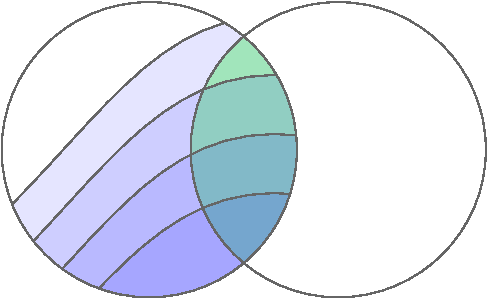
\includegraphics[width=10cm]{FoliationMarkov.pdf}};

%\begin{pgfonlayer}{background}
%\clip (180:1.6) circle (2.5cm);
%\fill[green!30] (0:1.6) circle (2.5cm);
%\end{pgfonlayer}

%\node[circle, draw=black!60, semithick, minimum size=2*\vennrad, inner sep=0, outer sep=0] (Past) at ($(split.north west) + (-0.9*\vennrad, 0.9*\vennrad)$) {};
%\node[circle, draw=black!60, semithick, minimum size=2*\vennrad, inner sep=0, outer sep=0] (Future) at (split.center) {};

\draw[draw=black!40, line width=1pt] ($(split.center) + (-\vennrad, \vennrad)$) circle (\vennrad);
\draw[draw=black!40, line width=1pt] (split.center) circle (\vennrad);

\begin{scope}
\clip ($(split.center) + (-\vennrad, \vennrad)$) circle (\vennrad);
\draw[fill=yellow, opacity=0.5] (split.center) circle (\vennrad);
\end{scope}

\draw[draw=black!50, line width=1pt] ($(split.center) + (-\vennrad, \vennrad)$) circle (\vennrad);
\draw[draw=black!50, line width=1pt] (split.center) circle (\vennrad);

% foliation
\begin{scope}
\clip ($(split.center) + (-\vennrad, \vennrad)$) circle (\vennrad);

\foreach \up in {3cm,2cm,1cm,0cm}{
\filldraw[draw=black!50, semithick, fill=green, fill opacity=0.1] ($(split.center) + (-2*\vennrad, \up)$) -- ++(0.666*\vennrad + \up, 0cm) -- ++(\vennrad,-\vennrad) -- ++(0cm, -\vennrad) -- ++(-3*\vennrad, 0cm) -- cycle;
% TODO: could use the control points to make foliation curved
%\filldraw[draw=black!60, semithick, fill=blue, fill opacity=0.1] ($(split.center) + (-\vennrad, \up)$) .. controls ++(-2,-2+\up) and (-1,0+\up) ..  (2,-1+\up) -- (3,0) -- (3,-5) -- (-3,-5) --   cycle;
}
\end{scope}

%%%% CONTACT
%\matrix[mat, anchor=south east,
%inner sep=5pt] (contact) at ($(split.north west) + (0.0cm, 0.0cm)$) {
%mohnjahoney@gmail.com\\
%(530) 601-0524\\
%\href{\mywebsite}{mohnjahoney.github.io}\\
%\node[draw=none, line width=3pt, rectangle] (gh) {
%\href{https://github.com/mohnjahoney}{
\includegraphics[width=0.6cm]{github.pdf}}
%\quad
%\href{https://www.linkedin.com/in/johnmahoney3}{
\includegraphics[width=0.6cm]{LI-In-Bug.png}}
%};\\
%};

%%% Profile
\matrix[sec_body_mat, anchor=south west, draw=strongblue,
column 1/.style={sec_text, text width=1.0*\bodywidth}] (profile) at ($(split.north east) + (0.0, +\sectionpad)$){
I'm a rad dad who endeavors to make the world a fizzier place. 
A physicist by training and jazz saxophonist by night, I approach the world with both an analytic mind and a the desire for a deep pocket.\\
};

\matrix[sec_title_mat, anchor=south west,
row 1/.style={sec_title, anchor=center}] (profile_title) at ($(profile.north west) + (0.0cm, +\sectionpad)$) {
\node[sec_title_circle] {};&
~~PROFILE~~&
\node[sec_title_circle] {};\\
};

%%% NAME other design
\node[color=white, fill=strongblue, font=\Huge, scale=2.0, anchor=south west] (name) at ($(profile_title.north west) + (0, +\sectionpad)$) {John R. \textcolor{yellow}{Mahoney}};

%\matrix[sec_title_mat, anchor=north west,
%row 1/.style={anchor=center}] (profile_title) at ($(split.south east) + (0.0cm, 0.0cm)$) {
%\node[draw=strongblue, circle, minimum width=0.3cm, anchor=center] {};&
%~~PROFILE~~&
%\node[draw=strongblue, circle, minimum width=0.3cm, anchor=center] {};\\
%};
%
%\matrix[sec_body_mat, anchor=north west, 
%column 1/.style={sec_text, text width=1.0*\bodywidth}] (profile) at ($(profile_title.south west) + (0.0, -\sectionpad)$){
%I'm a rad dad who endeavors to make the world a fizzier place. 
%A physicist by training and jazz saxophonist by night, I approach the world with both an analytic mind and a the desire for a deep pocket.\\
%};

%%% Communication Skills
\matrix[sec_title_mat, anchor=north west,
row 1/.style={sec_title, anchor=center}] (communication_skills_title) at ($(split.south east) + (0.0cm, -\sectionpad)$) {
\node[sec_title_circle] {};&
~~COMMUNICATION SKILLS~~&
\node[sec_title_circle] {};\\
};
%\matrix[sec_title_mat, anchor=north west,
%row 1/.style={anchor=center}] (communication_skills_title) at ($(profile.south west) + (0.0cm, -\sectionpad)$) {
%\node[draw=strongblue, circle, minimum width=0.3cm, anchor=center] {};&
%~~COMMUNICATION SKILLS~~&
%\node[draw=strongblue, circle, minimum width=0.3cm, anchor=center] {};\\
%};

\matrix[sec_body_mat, anchor=north west, 
column 1/.style={sec_bold, text width=0.2*\bodywidth},
column 2/.style={sec_text, text width=0.8*\bodywidth}] (communication_skills) at ($(communication_skills_title.south west) + (0.0, -\sectionpad)$){
Written: &  Wrote and co-authored over 25 papers published in high quality journals (PRL, PRX, PRA, PRE, CHAOS, J. Stat Phys.). Edited multiple articles for colleagues. Refereed for several journals.
Read about:
\href{https://mohnjahoney.github.io/pdfs/Times_Barbed_Arrow.pdf}{prediction}, 
\href{https://mohnjahoney.github.io/pdfs/A_Turnstile_Mechanism_For_Fronts_Propagating_In_Fluid_Flows.pdf}{reacting fluids}, 
\href{https://mohnjahoney.github.io/pdfs/Occams_Quantum_Strop.pdf}{quantum information}.\\
Verbal: & Designed and delivered over 35 talks and posters including:
Quantum Info Workshop at Nanyang Technical University, Singapore;
Conference on Complex Systems, Amsterdam;
CHAOS15 at Henri Poincar\'e Institute, Paris;
Oberwolfach, Germany (awarded \href{https://mohnjahoney.github.io/pdfs/posters/Oberwolfach2014.pdf}{``best poster''});
International Conference on Flow Dynamics, Sendai, Japan
%International Conference on Nonlinear Science and Complexity, Budapest, Hungary
% TODO: add "Listen to: link to a talk I've given."
\\
Graphical: & Value design and aesthetics in communication. I seek to balance precision and depth with clarity and impact. One significant output of my research on reacting flows is the graphical presentation of an augmented flow topology. My research in information theory was often facilitated by Venn diagrams, a technique I helped to incorporate in my research group. Sometimes, as with my study on self-propelled agents, the result is as much art as it is science.
Look at:
\href{https://mohnjahoney.github.io/images/burning_front_topology.png}{topology of reacting flows}, 
\href{https://mohnjahoney.github.io/images/FoliationCryptic.pdf}{info diagram}, 
%\href{https://mohnjahoney.github.io/images/quantum_strop_nemo.png}{quantum compression},
\href{https://mohnjahoney.github.io/images/poincare_mosaic.pdf}{Poincar\'e art}.\\
% TODO: add a video - maybe a BIM animation
%\phantom{blank} & Examples: \href{https://mohnjahoney.github.io/images/burning_front_topology.png}{A}, \href{https://mohnjahoney.github.io/images/quantum_strop_nemo.png}{B}, \href{https://mohnjahoney.github.io/images/poincare_mosaic.pdf}{C}\\
%\phantom{blank} & \node[draw=none] () {
%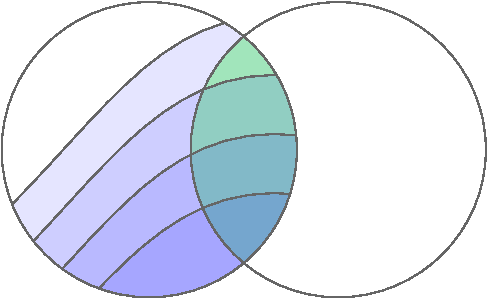
\includegraphics[width=2cm]{FoliationMarkov.pdf}
%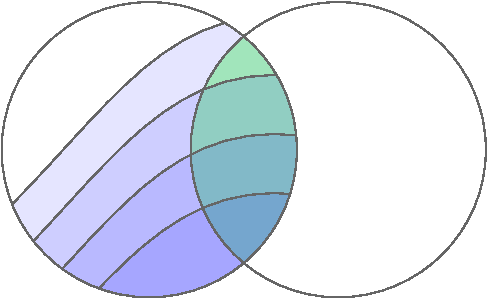
\includegraphics[width=2cm]{FoliationMarkov.pdf}};\\
};

%%% Analytic Skills
\matrix[sec_title_mat, anchor=north west,
row 1/.style={sec_title, anchor=center}] (analytic_skills_title) at ($(communication_skills.south west) + (0.0cm, -\sectionpad)$) {
\node[sec_title_circle] {};&
~~ANALYTIC SKILLS~~&
\node[sec_title_circle] {};\\
};

\matrix[sec_body_mat, anchor=north west, 
column 1/.style={sec_bold, text width=0.2*\bodywidth},
column 2/.style={sec_text, text width=0.8*\bodywidth}] (analytic_skills) at ($(analytic_skills_title.south west) + (0.0cm, -\sectionpad)$) {
Research: & Connected my work on reacting fluids to several existing fields: invariant manifolds, finite-time Lyapunov exponents, advection-reaction-diffusion equation, catastrophe theory, path planning in autonomous vehicles, differential geometry.\\
Critical Thinking: & Reframed an assumption in the literature to create a fruitful research avenue - \textit{crypticity and cryptic order}. \\
Data: & Created Python pipeline for data on diabetes patients: clean, process, analyze (multiple pair lagged regression), visualize. \\
};


%%% Work Experience
\matrix[sec_title_mat, anchor=north west,
row 1/.style={sec_title, anchor=center}] (work_experience_title) at ($(analytic_skills.south west) + (0.0cm, -\sectionpad)$) {
\node[sec_title_circle] {};&
~~WORK EXPERIENCE~~&
\node[sec_title_circle] {};\\
};

\matrix[sec_body_mat, anchor=north west, 
column 1/.style={sec_bold, text width=0.2*\bodywidth},
column 2/.style={sec_text, text width=0.8*\bodywidth}
] (work_experience) at ($(work_experience_title.south west) + (0.0cm, -\sectionpad)$) {
Fall 2020&Math Specialist: UC Davis\\
Summer 2020&Course Designer and Instructor: UC Davis\\
Oct 2019&Math Lecturer: Napa Valley College\\
Spring 2019&Physics Lecturer: UC Davis\\
Fall 2018&Math Lecturer: CSU Maritime\\
2017-2018&Consultant: Dept. Biomedical Informatics, Columbia University\\
Fall 2017&Spring 2018, Math Lecturer: UC Davis\\
2015-2017&Project Scientist: UC Davis\\
2010-2015&Postdoctoral Scholar: UC Merced\\
};


%%% Education
\matrix[sec_title_mat, anchor=north west,
row 1/.style={sec_title, anchor=center}] (education_title) at ($(work_experience.south west) + (0.0cm, -\sectionpad)$) {
\node[sec_title_circle] {};&
~~EDUCATION~~&
\node[sec_title_circle] {};\\
};

\matrix[sec_body_mat, anchor=north west,
column 1/.style={sec_text, anchor=west}, text width=\bodywidth] (education) at ($(education_title.south west) + (0.0cm, -\sectionpad)$) {
Ph.D. in Physics, UC, Davis with James P. Crutchfield\\
%�Extensions of the Theory of Computational Mechanics�
B.S. in Physics and Mathematics, CSU, Chico\\
attended Williams College for Physics, Mathematics and Music\\
};


%%%%%%%%%%%
% Sidebar
%%%%%%%%%%%

%%% Programming Skills
\matrix[sec_title_mat, anchor=north east,
row 1/.style={sec_title, anchor=center}] (programming_skills_title) at ($(split.south west) + (0.0cm, -\sectionpad)$) {
\node[sec_title_circle] {};&
~~PROGRAMMING~~&
\node[sec_title_circle] {};\\
};

%column 1/.style={font=\bfseries\Large, text width=0.2*\bodywidth},
%column 2/.style={text width=0.8*\bodywidth}
\matrix[sec_body_mat, anchor=north east, text width=\sidebarwidth, align=right, 
column 1/.style={sidebar_text, anchor=west}] (programming_skills) at ($(programming_skills_title.south east) + (0.0cm, -\sectionpad)$) {
Python: np, sp, mpl, pd\\
GUI / interactive\\
git, \LaTeX, beamer, tikz\\
ipython, Jupyter, VS Code\\
MATLAB\\
Mac OS, UNIX\\
};

%%% Interpersonal Skills
\matrix[sec_title_mat, anchor=north east,
row 1/.style={sec_title, anchor=center}] (interpersonal_skills_title) at ($(programming_skills.south east) + (0.0cm, -\sectionpad)$) {
\node[sec_title_circle] {};&
~~INTERPERSONAL~~&
\node[sec_title_circle] {};\\
};

\matrix[sec_body_mat, anchor=north east, text width=\sidebarwidth, align=right,
column 1/.style={sidebar_text}] (interpersonal_skills) at ($(interpersonal_skills_title.south east) + (0.0cm, -\sectionpad)$) {
Excellent listener\\
Flexible and creative\\
Work well in close-knit teams\\
Independent worker\\
Thoughtful mentor\\%: (3 PhD, 7 undergrads)\\
Value clear communication\\
};


%%% Projects
\matrix[sec_title_mat, anchor=north east,
row 1/.style={sec_title, anchor=center}] (projects_title) at ($(interpersonal_skills.south east) + (0.0cm, -\sectionpad)$) {
\node[sec_title_circle] {};&
~~PROJECTS~~&
\node[sec_title_circle] {};\\
};

\matrix[sec_body_mat, anchor=north east, text width=\sidebarwidth, align=right,
column 1/.style={sidebar_text}] (projects) at ($(projects_title.south east) + (0.0cm, -\sectionpad)$) {
\href{https://github.com/mohnjahoney/magnacules}{Python \& Physics course}\\
\href{link}{Burning Invariant Manifolds}\\
\href{link}{CMPy} contributor\\
\href{https://github.com/mohnjahoney/simpsons_paradox}{Simpson's Paradox}\\
\href{link}{timesquare}\\
this \href{https://github.com/mohnjahoney/resume}{resum\`e}\\
};


%%% INTERESTS
\matrix[sec_title_mat, anchor=north east,
row 1/.style={sec_title, anchor=center}] (interests_title) at ($(projects.south east) + (0.0cm, -\sectionpad)$) {
\node[sec_title_circle] {};&
~~INTERESTS~~&
\node[sec_title_circle] {};\\
};

\matrix[sec_body_mat, anchor=north east, text width=\sidebarwidth, align=right,
column 1/.style={sidebar_text}] (interests) at ($(interests_title.south east) + (0.0cm, -\sectionpad)$) {
jazz saxophone and piano\\
soccer, tennis, and hiking\\
cooking and eating delicious food!\\
};


\matrix[mat, anchor=north east, sidebar_text,
inner sep=3pt, draw=none, line width=2pt, fill=yellow, fill opacity=0.5, draw opacity=1.0, text opacity=1.0] (contact) at ($(interests.south east) + (0.0cm, -2*\sectionpad)$) {
mohnjahoney@gmail.com\\
(530) 601-0524\\
\href{\mywebsite}{mohnjahoney.github.io}\\
\node[draw=none, line width=3pt, rectangle] (gh) {
\href{https://github.com/mohnjahoney}{
\includegraphics[width=0.8cm]{github.pdf}}
\quad
\href{https://www.linkedin.com/in/johnmahoney3}{
\includegraphics[width=0.8cm]{LI-In-Bug.png}}
};\\
};


\end{tikzpicture}
\end{preview}
\end{document}
